\documentclass{llncs}

\usepackage{color}
\usepackage{colortbl}
\usepackage{epsfig}
\usepackage{listings}
\usepackage{array}
\usepackage{longtable}
\usepackage{hhline}
\usepackage{cite}
\usepackage{boxedminipage}
\usepackage{graphicx}
\usepackage{amsmath}

\newcommand{\notesbox}[1]{
  \noindent\begin{center}\begin{boxedminipage}[h]{0.4\textwidth}{#1}\end{boxedminipage}\end{center}
}

\definecolor{lightgray}{gray}{.95}
\definecolor{darkgray}{gray}{.80}

\lstset{
  lineskip=0.5pt,
  basicstyle=\scriptsize,             % the size of the fonts that are used for the code
  %numbers=left,                      % where to put the line-numbers
  numberstyle=\scriptsize,            % the size of the fonts that are used for the line-numbers
  stepnumber=1,                       % the step between two line-numbers. If it is 1 each line will be numbered
  numbersep=3pt,                      % how far the line-numbers are from the code
  backgroundcolor=\color{lightgray},  % choose the background color. You must add \usepackage{color}
  showspaces=false,                   % show spaces adding particular underscores
  showstringspaces=false,             % underline spaces within strings
  showtabs=false,                     % show tabs within strings adding particular underscores
  frame=none,                         % adds a frame around the code
  tabsize=2,                          % sets default tabsize to 2 spaces
  captionpos=b,                       % sets the caption-position to bottom
  breaklines=true,                    % sets automatic line breaking
  breakatwhitespace=false,            % sets if automatic breaks should only happen at whitespace
  escapeinside={\%}{)}                % if you want to add a comment within your code
}

\hyphenation{op-tical net-works semi-conduc-tor}

\begin{document}

\title{Automatically Repairing Concurrency Bugs\\ with ARC}

\author{David Kelk, Kevin Jalbert, Jeremy S. Bradbury}

\institute{Software Quality Research Laboratory\\
%Faculty of Science (Computer Science)\\
University of Ontario Institute of Technology\\
Oshawa, Ontario, Canada\\
\email{\{david.kelk, kevin.jalbert, jeremy.bradbury\}@uoit.ca}\\
\url{http://www.sqrlab.ca}}

\maketitle

\begin{abstract}

%Automatic program repair using search-based algorithms has been successfully applied to single-threaded programs. Similar progress has not been made on the automatic repair of concurrent programs. Several challenges exist in concurrent program repair  that are not found in sequential source code. Concurrent programs have many possible thread interleavings that make bugs harder to detect and concurrent programs have to contend with complex interaction bugs that do not appear in single-threaded source code.
In this paper we introduce ARC -- a fully automated system for repairing deadlocks and data races in concurrent Java programs. ARC consists of two phases: (1) a bug repair phase and (2) an optimization phase. In the first phase, ARC uses a genetic algorithm without crossover to mutate an incorrect program, searching for a variant of the original program that fixes the deadlocks and data races. As this first phase may introduce unneeded synchronization that can negatively affect performance, a second phase attempts to optimize the concurrent source code by removing any excess synchronization without sacrificing program correctness. We describe both phases of our approach and report on our results.
\keywords{concurrency, bug repair, evolutionary algorithm, SBSE, concurrency testing.}

\end{abstract}

 \section{Introduction}
\label{sec:introduction}

As computers and even mobile devices now ship with more than one core per chip, programs must parallelize~\cite{SL05} to take advantage of improvements in processing power. Improvements in clock speed alone won't save us anymore. Parallelism introduces a new class of bugs that are difficult to find because they may only occur in a small set of thread interleavings~\cite{MQB07}. Even when a concurrency bug has been detected, its repair is often non-trivial. Many concurrency bugs are the result of the interaction of different code fragments executing in different threads within a program. 

The use of search-based software engineering (SBSE)~\cite{Har+10} techniques to automatically repair bugs is not a novel idea~\cite{FNWG09, WNLF09, NWLF09, WFGN10, GNFW11, LDFW12}. To address the challenges of detecting and fixing concurrent programs we propose ARC (\textbf{A}utomatic \textbf{R}epair of \textbf{C}oncurrency bugs) -- an automatic technique to repair deadlocks and data races in concurrent Java programs. ARC requires no formal specifications, annotations or test suite. Only the Java source code and tests capable of demonstrating the deadlocks and data races are necessary. ARC works by using a genetic algorithm without crossover $(GA \neg C)$ to evolve variants of a incorrect concurrent Java program until one is found that fixes the bugs.

A common problem for automatic bug repair techniques is the large search space of possible fixes. Applying these techniques to  concurrent programs adds thread interleavings to the search space. ARC incorporates techniques to constrain the search space and make it tractable. First, we limit the algorithm to only fixing deadlocks and data races in concurrent Java programs. Second, ARC only targets concurrency mechanisms. \texttt{Synchronize} statements are added, removed, and manipulated. Third, we use a specific set of 12 TXL~\cite{CHP91} operators based on the ConMAn suite~\cite{BCD06} to mutate the program.  Fourth, the Chord tool~\cite{NA07} is used to perform a static analysis of the program to find and target the shared classes, methods and variables. This shared list is further refined by the ConTest tool. Fifth, ConTest is used to explore the interleaving spaces by applying noise to the interleavings selected.  Note that the framework is general enough to fix additional kinds of concurrency bugs and work on other programming languages. This evaluation is limited to fixing deadlocks and data races in Java programs.

In Section~\ref{sec:background} we cover background material related to concurrency and genetic algorithms. The motivation for ARC along with an example problem is presented in Sect.~\ref{sec:motivation}. In Section~\ref{sec:Phase1Functional} we describes how ARC evolves fixes for data races and deadlocks. Improving nonfunctioal properties of the program, such as its execution time is described in Section~\ref{sec:Phase2Nonfunctional}. We evaluate ARC in Section~\ref{sec:experiments} on a series of programs from the IBM benchmark. Threats to validity are discussed in Section~\ref{sec:threats}. In Section~\ref{sec:related_works} we discuss related works in the field of automatic program repair.  We conclude and present future work in Section~\ref{sec:conclusion}.

\section{Background}
\label{sec:background}

% TODO Possibly trim this sub-section?
%\subsection{Concurrency Bugs}
%\label{sec:concurrency}

%Data races and deadlocks are two of the most common concurrency bugs. A \textbf{data race} can be defined as: \textit{``\ldots two or more concurrent threads access a shared variable and when at least one access is a write, and the threads use no explicit mechanism to prevent the access from being simultaneous.''}~\cite{LSW07}. A \textbf{deadlock} can be defined as: \textit{``\ldots a situation where two or more processes are unable to proceed because each is waiting for one of the others to do something in a deadlock cycle \ldots} For example, a deadlock can occur when one thread in a program holds a lock that another thread desires and vice-versa''~\cite{LSW07}.

%Improper synchronization in concurrent Java programs allows data races and deadlocks to occur.  These bugs are extremely difficult to detect due to the non-deterministic nature of how threads are interleaved (i.e., the way the system schedules threads). Various techniques are available to detect concurrency bugs such as static analysis~\cite{NA07,NPSG09,HP04}, stress testing~\cite{HSU03}, dynamic analysis~\cite{JNPS09,EFN+02}, and model checking~\cite{BHPV00,RDH03,OM03,MQB07,Holz97,JM04,HP00}.


\subsection{Genetic Algorithms}
\label{sec:genetic_algorithms}

Genetic algorithms~\cite{GA92} (GAs) are a heuristic search technique modeled on natural evolution.  They are population based and uses mutation, crossover and a fitness function to evolve solutions to problems. Proposed solutions are encoded in individuals of the population. Each individual is evaluated by a fitness function, an equation that determines how close the individual is to the solving the problem. The more fit a individual's solution is, the greater the chance it will pass it's genetic material (i.e., itself) into the next generation. Crossover mixes the individuals to produce new ones while mutation injects fresh information in to the population so it does not become stagnant.

ARC uses a genetic algorithm without crossover (GA$\neg$C) and selection. A population of proposed solutions is generated in the first generation and mutated each generation. Two ending conditions exist.  First, a fix is found for the data races and deadlocks or a fixed number of generations pass with no solution found.

%Initially we rejected the use of crossover because of fears it would create mismatching synchronization blocks.  Upon reflection we believe this was a mistake.  We are looking at adding crossover to a future version of ARC.


\section{Motivation}
\label{sec:motivation}

\begin{figure}[t!]
\begin{minipage}{5cm}
\footnotesize{\textbf{Buggy Program:}}
\begin{lstlisting}[language=Java, morekeywords={synchronize}]
write(int var1){
  ... // Expensive loop
  data = var1;
  ... // Database query
}

int public read(){
  return data;
}
\end{lstlisting}
\end{minipage}\hfill
\begin{minipage}{5cm}
\footnotesize{\textbf{Fixed Program:}}
\begin{lstlisting}[language=Java, morekeywords={synchronize}]
synchronize write(int var1){
  ... // Expensive loop
  data = var1;
  ... // Database query
}

int synchronize read(){
  return data;
}
\end{lstlisting}
\end{minipage}
\caption{A developer first synchronizes the \texttt{read} function, yet the bug
still exists. Synchronizing the \texttt{write} method as well fixes the bug.}
\label{fig:fixed_sample_datarace}
\end{figure}

\begin{figure}[t!]
\begin{minipage}{5cm}
\footnotesize{\textbf{$1^{st}$ Optimization on Fix:}}
\begin{lstlisting}[language=Java, morekeywords={synchronize}]
public write(int var1){
 ... // Expensive loop
 synchronized(this){
   data = var1;
   ... // Database query
 }
}

int synchronize read(){
 return data;
}
\end{lstlisting}
\end{minipage}\hfill
\begin{minipage}{5cm}
\footnotesize{\textbf{$2^{nd}$ Optimization on Fix:}}
\begin{lstlisting}[language=Java, morekeywords={synchronize}]
public write(int var1){
 ... // Expensive loop
 synchronized(this){
   data = var1;
 }
 ... // Database query
}

int synchronize read(){
 return data;
}
\end{lstlisting}
\end{minipage}
\caption{A developer shrinks the critical region to exclude the expensive loop (Optimization 1). Next, a developer shrink the critical region again to exclude the database query (Optimization 2).}
\label{fig:optimized_sample_datarace}
\end{figure}


To illustrate the challenges of concurrency bug repair we consider an example of a data race and how ARC might fix it. In the left part of Figure~\ref{fig:fixed_sample_datarace} the \texttt{read} and \texttt{write} method access a shared variable. A very simple data race exists because there is no atomic access to the \texttt{data} variable during the concurrent reading or writing. A possible repair involves synchronizing both accesses as shown in the right part of Figure~\ref{fig:fixed_sample_datarace}. Note that synchronizing one method alone does not fix this bug. Section~\ref{sec:Phase1Functional} describes this in more detail.

The solution in the right part of Figure~\ref{fig:fixed_sample_datarace} is far from ideal. The solution found by ARC forces other threads to wait unnecessarily while the write method works in the loop and database sections. An optimization is to shrink the critical region guarded by the synchronize statements to only guard access to the shared variable as shown in Figure~\ref{fig:optimized_sample_datarace}.  Section~\ref{sec:Phase2Nonfunctional} describes how ARC attempts to optimize fixes found in the first phase of operation by removing and shrinking synchronization blocks. 

\section{Phase 1: Fixing Deadlocks and Data Races}
\label{sec:Phase1Functional}

ARC requires two inputs: An incorrect concurrent Java program and JUnit tests exercizing the errors. The test suite is the oracle that determines if bugs still exists in the program. One limitation of ARC (and of other related automatic bug fixing techniques mentioned in Section~\ref{sec:related_works}) is that it can only fix bugs detectable by the test suite. Given an incorrect program ARC performs a static analysis to identify the variables, classes and methods involved in concurrency.  It then invokes the GA$\neg$C to find fixes for the data races and deadlocks.  Each generation is broken down into a number of steps, shown in Figure~\ref{fig:Phase1GAnotC} and described here.

\begin{figure}[t!]
  \centering
  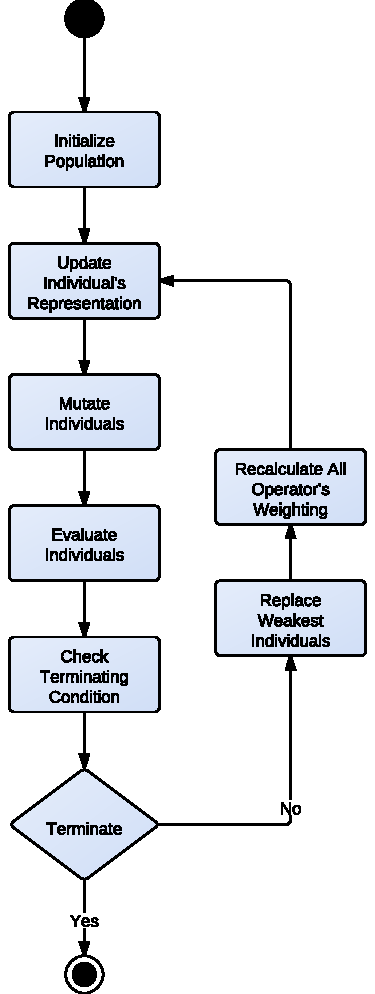
\includegraphics[width=7cm]{figures/phases.pdf}
  \caption{Detailed view of the GA$\neg$C used in Phase 1, the repair phase.}
  \label{fig:Phase1GAnotC}
\end{figure}

\subsection{Update Population}
\label{sec:UpdatePopulation}

First, the members of the population must be created.  If ARC has just started, the original incorrect program is replicated and copied into each member of the GA$\neg$C in the first generation.  For succeeding generations N the program for the same member from generation N - 1 is used. %This assures that each member of the population always works on their own copy of the program.

\subsection{Generate Mutants (Update Representation)}
\label{sec:GenerateMutants}

After the population is updated, ARC generates all mutants for all members using the operators in Table~\ref{tbl:Operators}.
These operators are implemented in  TXL~\cite{CHP91} using pattern matching and replacement rules. An example mutant created by the EXSB operator is shown in Figure~\ref{fig:EXSB_example}. 

\begin{table}[t!]
\caption{Set of mutation operators used by ARC.}
\begin{center}
\begin{tabular}{|l|l|c|c|}
\hline
\textbf{Operator Description} & \textbf{Acronym} \\
\hline
Add a synchronized block around a statement & ASAT \\
\hline
Add the synchronized keyword to the method header & ASIM \\
\hline
Add a synchronized block around a method & ASM  \\
\hline
Change the order of two synchronized blocks order & CSO  \\
\hline
Expand synchronized region after & EXSA  \\
\hline
Expand synchronized region before & EXSB  \\
\hline
Remove synchronized statement around a synchronized statement & RSAS  \\
\hline
Remove synchronization around a variable & RSAV  \\
\hline
Remove synchronized keyword in method header & RSIM  \\
\hline
Remove synchronization block around method & RSM  \\
\hline
Shrink synchronization block after & SHSA  \\
\hline
Shrink synchronization block before & SHSB  \\
\hline
\end{tabular}
\label{tbl:Operators}
\end{center}
\end{table}

\begin{figure}[t!]
\vspace{2mm}
\begin{minipage}{5cm}
\footnotesize{\textbf{ Program $P$:}}
\begin{lstlisting}[language=Java, morekeywords={synchronize}]
obj.write(var1);
synchronized(lock){
  myHash.remove(var1);
}
\end{lstlisting}
\end{minipage}\hfill
\begin{minipage}{5cm}
\footnotesize{\textbf{ Program $P'$:}}
\begin{lstlisting}[language=Java, morekeywords={synchronize}]
synchronized(lock){
  obj.write(var1);
  myHash.remove(var1);
}
\end{lstlisting}
\end{minipage}
\caption{An example of the EXSB (expand synchronization before) mutation operator.}
\label{fig:EXSB_example}
\end{figure}

\subsection{Apply a Mutation to an Individual}
\label{sec:mutate_individuals}

Once all mutants are generated for each individual, ARC selects a type of mutation (e.g. EXSB) and then an instance of it (e.g. 4$^{th}$ mutant generated) from those available. The selected mutation is copied into the source for the member. It is possible that the mutant isn't valid. For example, a new synchronization block could have been added that synchronizes on a variable that is out of scope. ARC attemps to compile the project.  If an error is detected, the mutation is rolled back and another is selected. This continues until a successful compilation or ARC runs out of mutants. In this latter case, ARC raises and exception and ends.

\subsection{Evaluate Individuals}
\label{sec:evalute_individuals}

A mutation may be beneficial, destructive or benign. We must evaluate it to determine it's effect on the program. A key problem in evaluating mutants is the unpredictability of thread interleavings. If a concurrency bug appears in only a few possible interleavings, how can we gain confidence that a proposed fix actually works? 

ARC uses IBM's ConTest tool~\cite{EFN+02} to instrument the software under repair by injecting noise into the selection of interleavings. This causes threads to randomly delay at different times during execution, increasing the chance that different interleavings are explored. By running the instrumented version of the program multiple times we gain more confidence that a larger set of the interleavings are explored. Choosing the number of times ConTest run to test each proposed fix is the most crucial parameter in ARC.  Confidence in any proposed fix must be carefully balanced against the time required to find the fix.

The number of successful ConTest executions are used to determine fitness:
\newline
\begin{footnotesize}
\begin{center}
$functional\ fitness(P) = (s \times sw) + (t \times tw)$
\end{center}
\end{footnotesize}
\begin{scriptsize}
\begin{center}
$s = \#\ of\ successful\ executions$ \\
$sw = success\ weighting$ \\
$t = \#\ of\ timeout\ executions$ \\
$tw = timeout\ weighting$
\end{center}
\end{scriptsize}

\noindent When determining fitness we consider both a successful execution and a timeout as positive factors. Timeouts are positive because given more time an execution that timed out may have resulted in a successful execution. We weight timeouts less than a successful execution though as the successful execution isn't guaranteed.

If ARC finds an individual that achieves 100\% successful executions, we need to ensure it is truly a fix. It is possible that a proposed solution could still contain a bug that escaped detection because the interleaving exhibiting it were not selected by ConTest. To increase our confidence that a fix is correct we take the base number of ConTest runs (say 10) and multiply it by an additioal safety factor (say 20). We run the proposed fix through ConTest ($10 \times 20 = 200$) more times to give us additional confidence the fix holds.  If a data race or deadlock is found during these additional runs, the fix is rejected and the search continues. This continues until a correct program is found or the GA$\neg$C runs out of generations.

\subsection{Replace Weakest Individuals}
\label{sec:replace_weakest_individuals}

We believe the \textit{competent programmer hypothesis}~\cite{ABD+79} applies when fixing concurrency errors.  That is, that programmers strive to create correct programs.  Programs with bugs in them are nearly correct so the distance in the search space from an incorrect program to a correct program is small(er) and tractable.  Even with a smaller search space, evolutionary alogirthms may evolve candidate solutions that stray down paths leading to little or no improvement. To encourage individuals to explore more fruitful areas of the state space we include the option to restart or replace the lower $w$ percentage (say 10\%) of individuals if they underperform for too long.  Two replacement strategies are used. First, the underperforming member is replaced with a random individual from the upper $x$ percent of the population. Second, the member is replaced by the original incorrect program.

\subsection{Recalculate Operator Weighting}
\label{sec:recalculate_operator_weighting}

ARC leverages historical information on how successful different mutation operators have been and about the relative dominance of data races and deadlocks. We give additional weight to operators that have raised the fitness of the population or reduced the frequency\footnote{For example, if EXSB reduces the occurrence of deadlocks from 80 of 100 ConTest runs to (say) 60 of 100 runs, it will be selected more frequently in future generations to combat deadlocks.} of data races or deadlocks.   The weighting is designed to ensure the chance of selecting an operator is always greater than zero regardless of their performance. Separate weightings are used for data races and deadlocks. A sliding window of $n$ generations is used to adapt the operator weighting to recent history. 

\section{Phase 2: Optimizing Fixes From Phase 1}
\label{sec:Phase2Nonfunctional}

ARC may introduce unnecessary synchronization during the fixing process. If a fix is found, an optional second phase begins that attempts to improve the running time of ARC by shrinking and removing unnecessary synchronization blocks.  The same strategy is used from part one.  A new fitness function and a subset of the TXL operators (RSAS, SHSA, ... from Table~\ref{tbl:Operators}) are used. 

\begin{footnotesize}
\begin{center}
$non-functional\ fitness(P) = \frac{worst\ score}{[sig_t \times unc(t)] + [sig_c \times unc(c)]}$
\end{center}
\vspace{0.1cm} \textit{Where:} \vspace{0.1cm}
\end{footnotesize}
\begin{scriptsize}
\begin{center}
$unc(x) = \frac{(x_{max} - x_{min})}{x_{avg}}$ \\ \vspace{0.2cm}
$
 sig_t = \left\{
 \begin{array}{l l}
   t/c & \quad if\ t\ > c \\
   c/t & \quad if\ c\ > t \\
 \end{array} \right.
$ \\ \vspace{0.2cm}
$
 sig_s = \left\{
 \begin{array}{l l}
   c/t & \quad if\ t\ > c \\
   t/c & \quad if\ c\ > t \\
 \end{array} \right.
$ \\
\end{center}
\end{scriptsize}

\noindent The fitness function depends on the real time, t, required for an execution and the number of voluntary context switches made, c.  Voluntary context switches is the number of times a thread voluntarily gives up control of the CPU. By minimizing unnecessary synchronization both of these values should decrease. At the beginning of phase 2 we run the correct, unoptimized program (without ConTest) a number of times to acquire the unoptimized running time and number of context switches. These values are used in the fitness function to evaluate relative improvements. 

Removing and reducing synchronization runs the risk of introducing new errors into the program. Before every non-functional evaluation we need to ensure that no bugs are present. We re-run the first phase's correctness check (eg, 10 ConTest runs, then 200 more). If any deadlocks or data races are encountered the proposed optimization is rejected and this individual is reset to the previous generation. After ARC validates the proposed optimization additional runs are conducted without using ConTest to obtain the running time and voluntary context fixes. 

Unlike phase 1 there is no early stopping criteria as there is no correct running time.  Lower is always better.  Phase 2 always uses its full allotment of generations. For this reason, running phase 2 is user-configurable.  Optimization of this phase is future work.

\section{Evaluation}
\label{sec:experiments}

In order to evaluate ARC's ability to repair concurrency bugs we selected 8 programs from the IBM Concurrency Benchmark~\cite{EHSU06}. We chose six programs containing bugs ARC can fix and two ARC cannot fix as a sanity check.

\begin{table}[h]
\caption{The set of programs from the IBM benchmark used to evaluate ARC.}
\begin{center}
\begin{tabular}{|l|r|r|l|l|p{4.5cm}|}
\hline
\textbf{Program} & \textbf{SLOC} & \textbf{Classes} & \textbf{Bug Type} & \textbf{Can Fix?}\\
\hline
account & 165 & 3 & Data Race & Yes\\
\hline
accounts & 75 & 2 & Data Race & Yes\\
\hline
bubblesort2 & 104 & 2 & Data Race & Yes\\
\hline

deadlock & 109 & 2 & Deadlock & Yes\\
\hline
lottery & 157 & 2 & Data Race & Yes\\
\hline
pingpong & 143 & 4 & Data Race & Yes\\
\hline
airline & 93 & 1 & Data Race & No\\
\hline
buffer & 319 & 5 & Data Race & No\\
\hline
\end{tabular}
\label{tbl:used_programs}
\end{center}
\end{table}

ARC is designed to be flexible. Table~\ref{tbl:used_parameters} describes the configuration options and values used in our evaluation. Parameter values are influenced by standards developed by the community (e.g., Evolution population, evolution gen.) and through experience gained using ARC (e.g., ConTest Runs, Validation Mult.). Of importance, the GA$\neg$C population size and generation size are both 30.  Every member at every generation is evaluated by being run through ConTest 10 times.  Any potential fix is evaluated 150 more times. Testing was conducted on a Linux PC with a 2.33 GHz processor, 4 gigabytes of RAM running Linux Mint 13.

% TODO Maybe reduce this to the commonGA parameters?
\begin{table}[t!]
\caption{The set of parameters that ARC uses along with their descriptions and values.}
\begin{center}
\lstset{basicstyle=\scriptsize}
\begin{tabular}{|l|p{7.5cm}|r|}
\hline
\textbf{Parameter} & \textbf{Description} & \textbf{Value}\\
\hline
Project Test MB & The amount of memory allocated  & 2000\\
\hline
ConTest Runs & Test suite executions per gen. per member & 10\\
\hline
Validation Mult. & Multiplier on ConTest runs when validating potentially correct programs & 15\\
\hline
Timeout Mult. & Time multiplier for ConTest before timeout & 20\\
\hline
Evolution Gen & Maximum number of generations of the GA$\neg$C & 30\\
\hline
Evolution Population & Population size for the GA$\neg$C & 30\\
\hline
Replace Lowest \% & Lowest $n$\% of population replaced in GA$\neg$C & 10\\
\hline
Replace With Best \% & Replace underperfomers with best individuals $n$\% of the time & 75\\
\hline
Replace min turns & Minimum time underperforming & 3\\
\hline
Replace Interval & Every $n$ generations, underperformers are replaced & 5\\
\hline
Ranking Window & Size of sliding window for operator weighting & 5\\
\hline
Success Weight & Fitness score for successful executions & 100\\
\hline
Timeout Weight & Fitness score for timeout executions & 50\\
\hline
Improv. Window & Number of generations to consider for convergence & 10\\
\hline
Avg. Fit. Delta & Minimum average fitness improvement required & 0.01\\
\hline
Best Fit. Delta & Minimum best fitness improvement required & 1\\
\hline
\end{tabular}
\label{tbl:used_parameters}
\end{center}
\end{table}

\subsection{Experimental Results}
\label{sec:experimental_results}

\begin{table}[t!]
\caption{Summary of the results of running the programs through ARC 5 times.}
\begin{center}
\lstset{basicstyle=\scriptsize}
\begin{tabular}{|l|l|l|}
\hline
\textbf{Program} & 
\textbf{Avg. Gen. Fix Found} & 
\textbf{Avg. Time Taken} 
\\\hline
account & 5 & 8m 8s
\\\hline
accounts & 1 & 44m
\\\hline
bubblesort2 & 2.2 & 1h 40m 20s
\\\hline
deadlock & 1 & 2m 12s
\\\hline
lottery & 2.4 & 38m
\\\hline
pingpong & 1 & 12m 32s
\\\hline

\end{tabular}
\label{tbl:summary_results}
\end{center}
\end{table}

Each program in Table~\ref{tbl:used_programs} was run through ARC 5 times using the parameters described in Table~\ref{tbl:used_parameters}. Results are summarized in Table~\ref{tbl:summary_results}. ARC was able to fix the 6 fixable programs and wasn't able to fix the 2 non-fixable. For the 6 repairable programs the time taken to find a fix ranged from about 2 minutes to 100 minutes. The most time consuming aspect of ARC is the numerous ConTest executions. Second is the waiting necessary to determine the difference between a successful execution and a timeout caused by a deadlock. The \textit{Timeout Multiplier} in Table~\ref{tbl:used_parameters} allows ARC to wait up to 20 times the instrumented execution time for the program to complete.

Almost all fixes are found in the first or second generation.  The static analysis by Chord and the dynamic analysis by ConTest significantly shrink the state space.  For example, the account program contains 3 classes, approx. 9 methods and 6 variables.  After the analysis, this is reduced to 2 classes, 3 methods and 3 variables.  A population of 30 may exceed the number of mutations available, leading to the search space probably being exhaustively covered.  If the correct program is 1 or 2 mutation steps from the incorrect one, it should be found quickly.  ARC works as a proof of concept and must be further evaluated -- more runs and on larger programs.

\section{Threats to Validity}
\label{sec:threats}

The main threat to validity for our experimental evaluation of ARC is external validity -- our ability to generalize results. Although we have used third-party programs in our evaluation, all of them are small and are not representative of large-scale concurrent software. In the future, we plan to address this threat by conducting further experiments with larger concurrent software systems.

\section{Related Works}
\label{sec:related_works}

Several approaches to sequential program repair have been proposed in the literature. For example, co-evolutionary competition between programs with bugs and between test cases~\cite{AY08, Arc08, WT10}. These approaches require formal specifications and use genetic programming to evolve fixes. Alternatively the work in requires no formal specifications. Instead, test cases are used to demonstrate the bug and describe the desired functionality that must be preserved. To address the limitations of the previous approach they introduce two innovations: First, they assume the bug is written correctly in another part of the program. Second, they determine the error path on which the bug occurs and target those statements specifically for repair. Together these additions constrain the state space enough that the framework can fix real bugs in real programs~\cite{FNWG09, WNLF09, NWLF09, WFGN10, GNFW11, LDFW12}.

For concurrent programs, there are several examples of related work. Similar to the work done here, ConTest is used to heal data races~\cite{KLT+07, LVK08}. Healing a program is not the same as repairing a program -- \textit{``The healing techniques based on influencing the scheduling do not guarantee that a detected problem will really be completely removed, but they can decrease the probability of its manifestation.''}~\cite{LVK08}. SAT solving~\cite{AY07}  is used to repair shared memory concurrent programs where processes atomically read and write one shared variable at a time. This work requires the concurrent program and a formal temporal logic specification. 

AFix~\cite{JSZL+11} is a framework for fixing single-variable atomicity violations. This approach combines dynamic bug analysis, patch creation and merging and dynamic testing. It is limited to manipulates mutex locks, works only with CTrigger and offers no guarantees of correctness.  They must use noising and dynamic analysis to determine if any deadlocks remain.  
Others have reported, \begin{quote}``Our evaluation of AFix on large real systems also shows that the AFix sometimes incurs the degraded performance and, worse, frequent deadlocks.~\cite{LZ12}''\end{quote}. Axis~\cite{LZ12} uses a branch discrete control theory called supervision based on place invariants to fix any number of correlated atomicity violations with minimal harm to concurrency. Their approach doesn't appear to be able to fix deadlocks though, as they state,  \begin{quote}``... guarantee that, if the original program is deadlock-free, our solution does not cause the patched program to deadlock~\cite{LZ12}.''\end{quote}

\section{Conclusions and Future Work}
\label{sec:conclusion}

We've introduced ARC, a framework to automatically repair deadlocks and data races in concurrent Java programs. Experiments were conducted to evaluate ARC using a set of 8 programs drawn from the IBM concurrency benchmark. ARC was able to fix the data races and deadlocks in all 6 of the fixable programs.

Although ARC was successful with the set of small programs from the IBM concurrency benchmark we still need to evaluate ARC's scalability on larger open source projects. In addition to scalability. To maximize the efficient use of ConTest we plan to explore different heuristics for seeding noise and different optimizations supported by ConTest~\cite{KLVU10}.


Finally, we plan to experiment with new mutation operators. Potential additions include splitting or merging synchronization blocks and adding new locks. Through experimentation we plan to optimize the existing set of mutation operators to maximize their capabilities.  Furthermore, we would like to expand ARC's operators to deal with new anti-patterns~\cite{BJ09, FKLV12, BCD06} and give ARC the ability to fix additional types of bugs.

\bibliographystyle{splncs03}
\bibliography{ARC2013}

\end{document}
